\begin{figure}
                \begin{subfigure}[b]{0.5\textwidth}
                    \centering
            %\centering
                    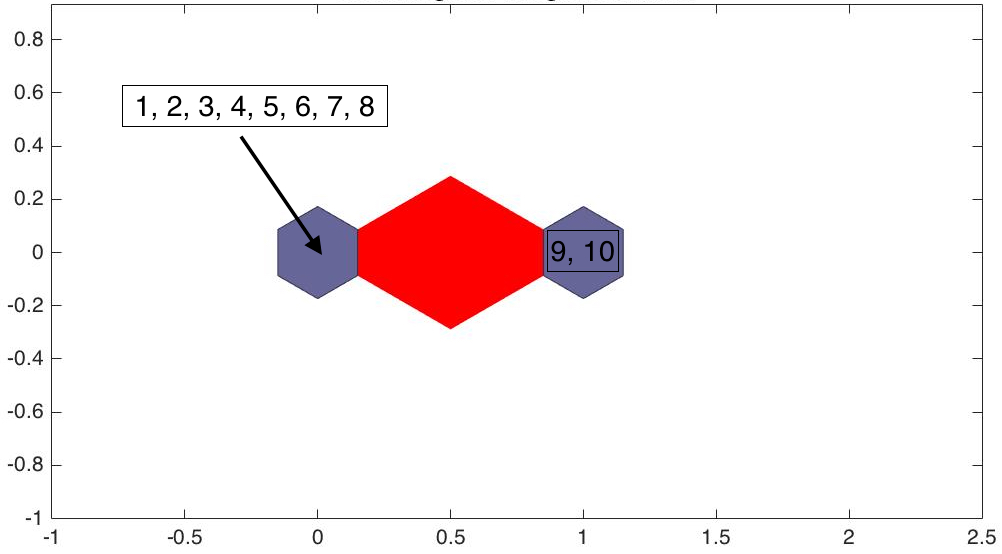
\includegraphics[width=\textwidth]{../images/M31/all/dist1by2.jpeg}
                    \caption{$1\times2$}
                     \label{fig: 1by2all}
                \end{subfigure}
                \hfill
                \begin{subfigure}[b]{0.5\textwidth}
                     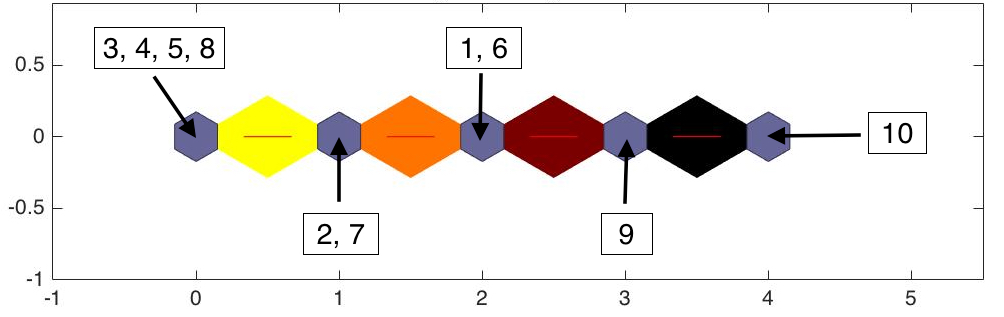
\includegraphics[width=\textwidth]{../images/M31/all/dist1by5.jpeg}
                     \caption{$1\times5$}
                     \label{fig: 1by5all}
                \end{subfigure}
                \hfill
                \hfill
                \begin{subfigure}[b]{0.5\textwidth}
                     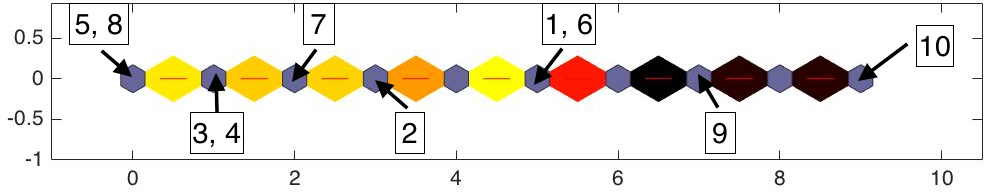
\includegraphics[width=\textwidth]{../images/M31/all/dist1by10.jpeg}
                     \caption{$1\times10$}
                     \label{fig: 1by10all}
                \end{subfigure}
                \caption{1D results from all data}
            \end{figure}

            \begin{figure}
                \begin{subfigure}[b]{0.5\textwidth}
                    \centering
                    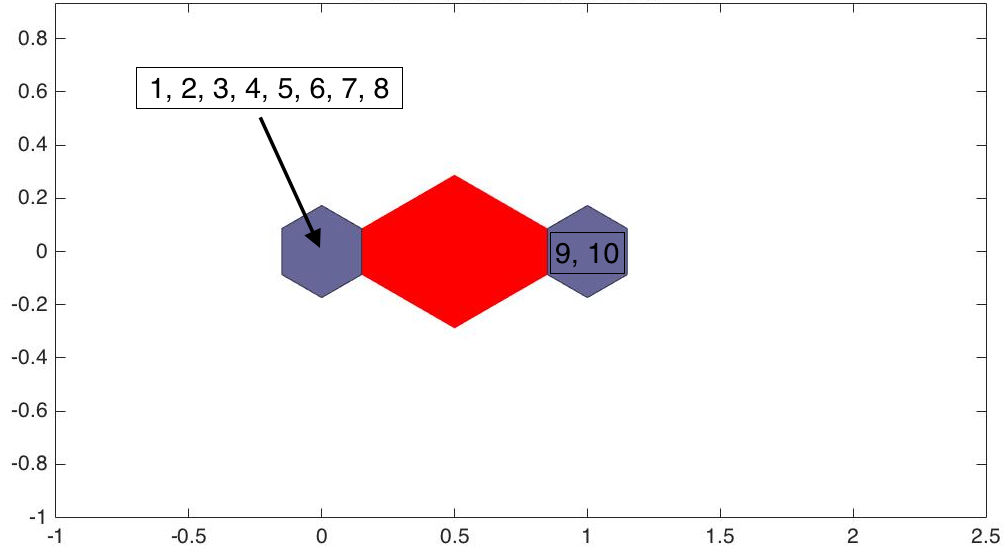
\includegraphics[width=\textwidth]{../images/M31/derived_ones/dist1by2.jpeg}
                    \caption{$1\times2$}
                    \label{fig: 1by2derived}
                \end{subfigure}
                \hfill
                \begin{subfigure}[b]{0.5\textwidth}
                    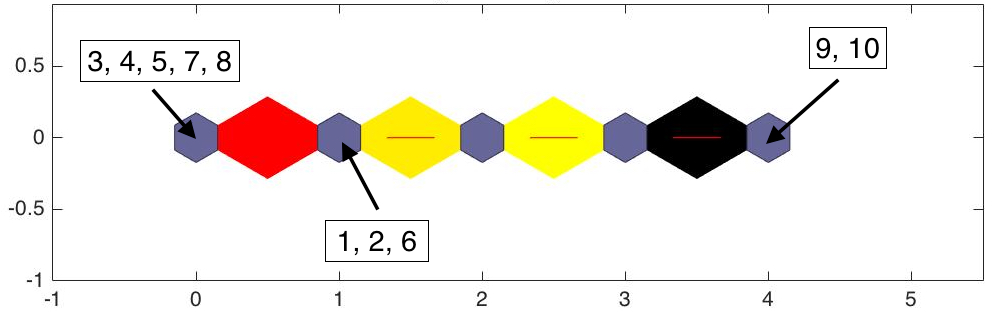
\includegraphics[width=\textwidth]{../images/M31/derived_ones/dist1by5.jpeg}
                    \caption{$1\times5$}
                    \label{fig: 1by5derived}
                \end{subfigure}
                \hfill
                \hfill
                \begin{subfigure}[b]{0.5\textwidth}
                    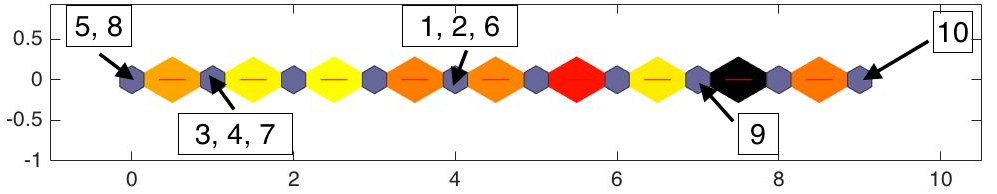
\includegraphics[width=\textwidth]{../images/M31/derived_ones/dist1by10.jpeg}
                    \caption{$1\times10$}
                    \label{fig: 1by10derived}
                \end{subfigure}
                \caption{1D results from derived ones}
                \label{fig: 1Dsoms}
            \end{figure}